\section*{Management and Coordination Plan}

% - 3 page limit

 \subsection*{Overall Management Structure}
 \begin{wrapfigure}{R}{0.6\textwidth}
  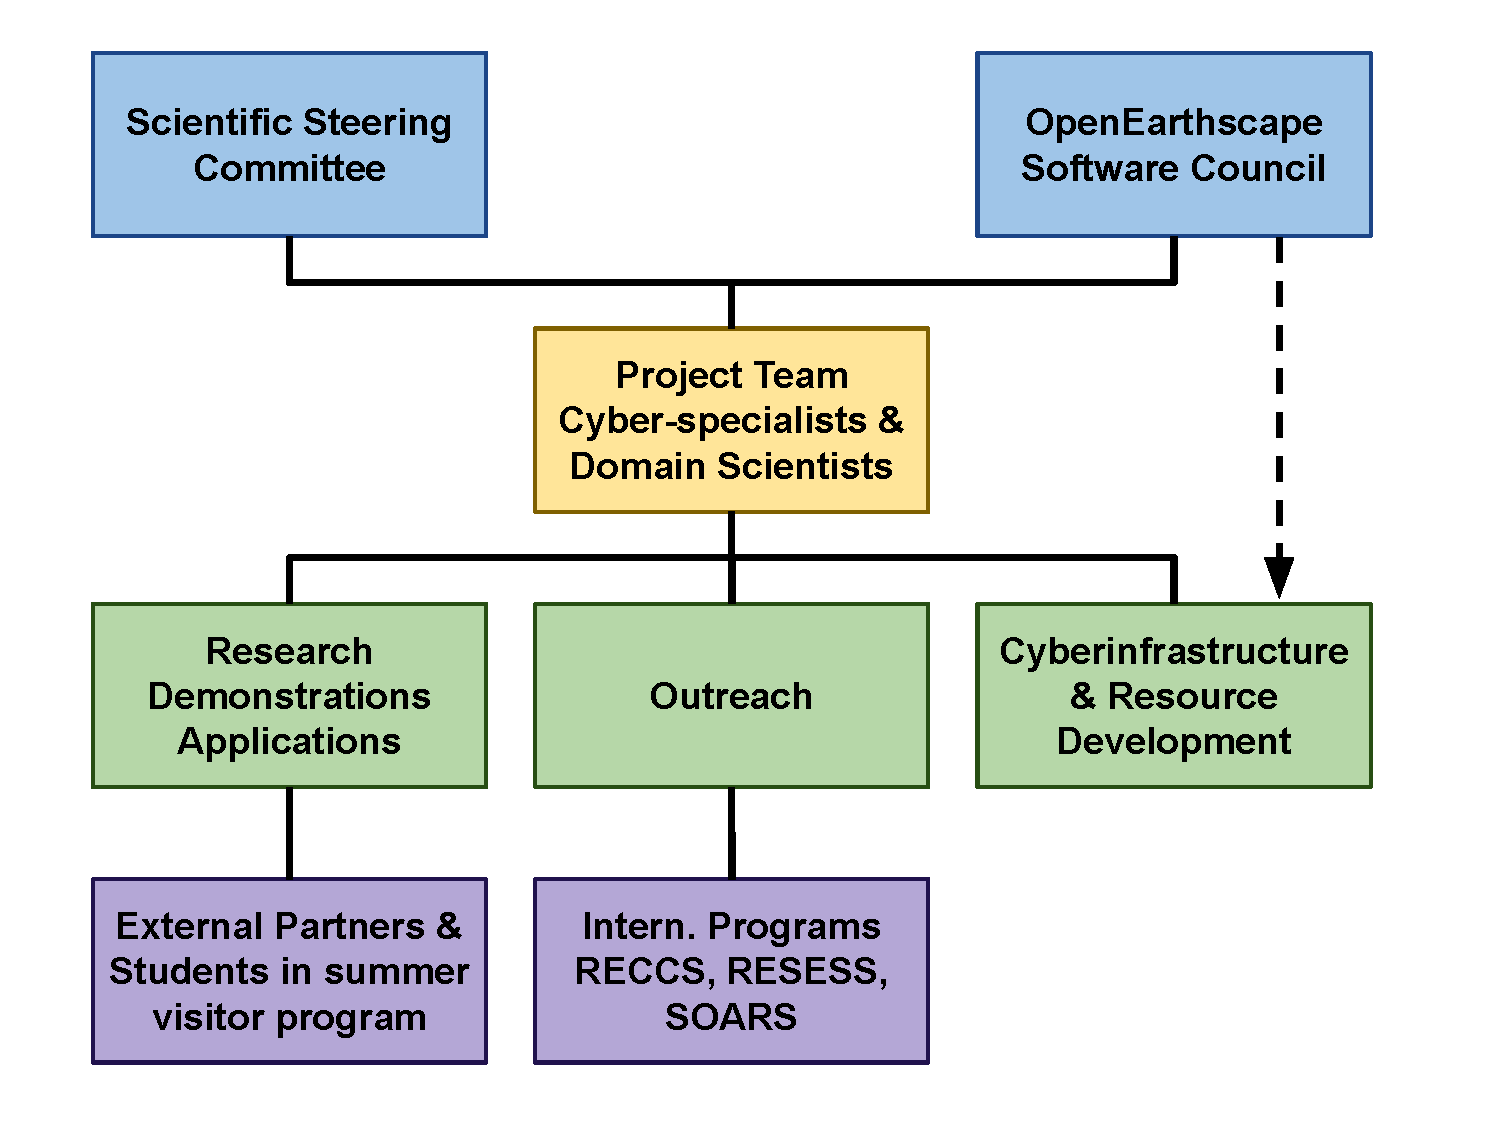
\includegraphics[width=0.6\textwidth]{OrgChart-4.pdf}
  \caption{Organizational structure for proposed project.}
  \label{fig:org-chart}
\end{wrapfigure}

Figure~\ref{fig:org-chart} shows the overall organizational structure. The Lead PI will oversee the management and coordination of the project.  In Year 1 a Scientific Steering Committee (SSC) will be formed. The SSC will meet annually (remotely) and will be responsible for advising on strategic planning, review of project metrics, evaluation of science demonstration projects, assessment of competing objectives, and needs of the project.  The SSC will include representatives of key community organizations and projects (such as the Open Modeling Foundation, the Consortium of Universities for the Advancement of Hydrologic Science [CUAHSI], Critical Zone Research Network, OpenTopography, and Computational Infrastructure for Geodynamics [CIG]).  Also in Year 1, an OpenEarthscape Software Council will be formed to guide software development and oversee long-term sustainability of specific products.  The Council will include interested members of the community, such as researchers from USGS, the Netherlands eScience Center, and Deltares. The Research Demonstration Applications, Cyberinfrastructure and Resource Development and Outreach deliverables teams will report to the Project Team.  The external partners and students participating in the summer visitor program will contribute to the Research Demonstration Applications team. The CU Boulder team will work with the directors of the 3 internship programs to coordinate the OpenEarthscape contributions.

\subsection*{Roles of the PI, co-PIs and Other Senior Personnel}
Key personnel essential for the management and completion of the proposed project are summarized below. Additional details regarding FTEs and specific job responsibilities are included in the Budget Justification. \textbf{Principal Investigator Dr.\ Gregory Tucker} will have overall responsibility for the project and will be engaged in supervision of personnel and all aspects of the project planning, implementation, deliverables, and reporting. Professor Tucker has a history of successful management of large research teams.  \textbf{Co-PI and Chief Research Software Engineer Dr.\ Eric Hutton} will apply his long history of successful scientific software development and management to the day-to-day project direction. He will conduct software design and development, particularly regarding PyMT and Landlab.  \textbf{Co-PI and Geospatial and Web Services expert Dr.\ Albert Kettner} will be responsible for web portal engineering as well as software management, especially with regard to hydrological models.  \textbf{Co-PI Dr.\ Irina Overeem} will be responsible for the research demonstration project on Arctic hydrology and geomorphology.  \textbf{Co-PI Dr.\ Julia Moriarty} will be responsible for the research demonstration project on cross-shelf sediment transport.  \textbf{Research Associate Dr. Peckham} will oversee implementation of the Scientific Variables Ontology, developing cross-framework compatibility tools and resources for the Basic Model Interface, and consulting on hydrologic modeling.  \textbf{Research Associate Dr.\ Maria Stoica} will be responsible for implementing the Scientific Variables Ontology and related supporting technology.  \textbf{Research Associate Dr.\ Chris Jenkins} will be responsible for guiding the research demonstration project on linking the dbSEABED seafloor dataset with models of carbon exposure to seabed erosion.  \textbf{Postdoctoral Research Associate (TBD)} will be responsible for producing use-case demonstrations that illustrate how the technology can be applied in the scientific domains represented by the project.  \textbf{Research Associate (TBD)} will be responsible for %integration and mediation of existing standards, 
software development/management, and computing workshops for the summer internship program. \textbf{Program Coordinator, Lynn McCready} will be responsible for general administrative management and logistical coordination. Other Project Assistants include an accounting tech and a systems administrator.

\subsection*{How the project will be managed across institutions and disciplines}
The project team already has a history of successfully working together across institutions and disciplines.  The following methods will be used for team coordination:
 
\begin{itemize}
\item Organizing biweekly remote Zoom meetings that will be held with all participants on the project, including graduate students, postdoctoral scholars, and other team personnel.
\item Annual goals will be set and revisited, together with analysis of metrics, approximately bimonthly during the project Remote Zoom meetings.
\item Branches and Pull Requests will be used for development on GitHub. To ensure quality control, he project repositories will be equipped with Continuous Integration using Travis and AppVeyor. %so that unit tests will automatically be triggered, and team members can ensure that the code that they are putting back into the repository will not create problems for other users.
\item Issue tracking on GitHub will allow team members and users to post questions, comments and issues, creating an open forum for all users to learn from one another.  Posted issues will alert team members when there are bugs or bottlenecks in certain parts of the code.
\end{itemize}
As described in the first section of the Management and Coordination Plan, the co-PIs will take the lead on reaching out to and including users and organizations from different disciplinary foci and in project modeling efforts. %Each PI/co-PI and will be responsible for updating the team on the needs of different users during the remote Zoom meetings.

\subsection*{Coordination mechanisms for cross-institution, cross-discipline scientific integration}
Beyond the regular remote Zoom meetings, there will be \textbf{yearly project meetings} of the PIs, graduate students, postdoctoral scholars and other senior personnel.  This annual meeting will be held in conjunction with the American Geophysical Union (AGU) Fall meeting, if public health considerations allow.  These meetings will be critical for brainstorming, setting new goals, refining old goals, and dealing with the types of problems that are not fixed within an hour-long Zoom discussion.  The in-person meetings will offer further opportunity for the team to learn about and take advantage of on-going cross-disciplinary efforts.
 
Users from other disciplines will be targeted through \textbf{OpenEarthscape clinics at disciplinary meetings}. Venues targeted include the Community Surface Dynamics Modeling System (CSDMS), Geological Society of America (GSA), American Geophysical Union (AGU), European Geosciences Union (EGU), the Earth Surface Processes Summer (ESPIn) Summer Institute, and CUAHSI meetings. This list may expand depending on user interests and opportunities.
 
Before they seek out OpenEarthscape clinics, users first need to know about the project, and \textbf{team members will present research at annual AGU and GSA meetings, which attract a broad range of earth scientists}.  Team members will submit abstracts to sessions with broad audiences and/or with varying disciplinary foci.  The team will also attend disciplinary meetings when appropriate to reach a broader scientific audience.

\textbf{The lead institution will also support travel plus stipend for 3 visiting student scientists per summer in Years 1--4 to gain hands-on, on-site training.} Each student visitor may request travel for one advisor to join them in Boulder for up to two weeks to work with the student and OpenEarthscape team. %We will require a short (one page) proposal from prospective visitors about the scientific questions that they wish to address using the proposed modeling framework.

\subsection*{Budget Items supporting project management and coordination}
 
Funding is included in the budget from each institution to support travel to conferences in which clinics will be given. Each PI has included funds to attend the AGU meeting, in conjunction with the OpenEarthscape team annual meeting.
 The lead PI has included funds to attend some additional meetings in order to advertise the OpenEarthscape project.
 Funding is included in the lead institution's travel budget to support 3 visiting graduate students for 3 months (summer) per year and 3 advisor visits for 2 weeks (summer) per year.

\subsection*{Year by year goals}

The schedule below designed as a preliminary plan, subject to evolution in response to project needs and external developments. We expect to be responsive in particular to the visiting graduate students, whose needs will guide priorities for the development of tools, templates, and tutorials.

\scitem{Year 1:} Establish OpenEarthscape Council. Prototype  EarthscapeHub. BMI for Julia. Tutorials on use of SVO, and on coupling agent-based and process models. Tutorial on reproducibility with WholeTale. Parallel-capability metadata for PyMT. Landlab marine components. Scientific computing workshops for undergraduate internship programs. Visiting grad student program.

\scitem{Year 2:} Release and market EarthscapeHub. BMI for  SVO-assistance resource. BMI for  WRF-Hydro. \texttt{CoupledModel} base class for PyMT components. Landlab \texttt{GlobalGrid} class. First version of BMI parallel extensions. Visualization pathways (utilities and  tutorials). Summer  computing workshops; visiting grad student program.

\scitem{Year 3:} BMI for Octave. Best-practice community guide and tutorial for building reproducible computational science packages via WholeTale. Search capability for SVO. BMI for SiSTER. Test coupling of geodynamic and surface process models using enhanced BMI. Refactor Landlab core routines to use Dask under-the-hood parallelization of vectors operations. Summer  computing workshops; visiting grad student program.

\scitem{Year 4:} 
Apply BMI for an agent-based model (e.g., NetLogo, Mesa). Develop updated version of BMI parallel extensions. Tool for interactive generation of Standard Names. Wrap TopoFlow hydrologic model components with BMI. Develop, demonstrate, and document Landlab \texttt{GlobalGrid} class. Revise best-practice guides and tutorials for reproducibility, in light of team and student experiences. Summer  computing workshops; visiting grad student program.

\scitem{Year 5:} 
BMI extension for data assimilation. Landlab \texttt{Grid3D} class. Design and launch of post-project sustainability program with OpenEarthscape Council. Manuscripts describing findings from research demonstration projects and technology development. Summer  computing workshops.

